\documentclass[11pt]{exam}

\usepackage{amsmath, amssymb, multicol}
\usepackage{graphicx}
\usepackage{textcomp}
\usepackage{skak} %for chessboards etc.
\usepackage[top=.75in, bottom=.25in, left=1in, right=1in]{geometry}
\usepackage{tikz}

\def\d{\displaystyle}
\def\b{\mathbf}
\def\R{\mathbf{R}}
\def\Z{\mathbf{Z}}
\def\st{~:~}
\def\bar{\overline}
\def\inv{^{-1}}


%\pointname{pts}
\pointsinmargin
\marginpointname{pts}
\addpoints
\pagestyle{head}
%\printanswers

\firstpageheader{Math 228}{\bf Counting Rook Paths}{Monday, Oct 1}


\begin{document}

%space for name
%\noindent {\large\bf Name:} \underline{\hspace{2.5in}}
%\vskip 1em

% \centerline{{\bf Math 228}}
\vskip 1em
In chess, a rook can move only in straight lines (not diagonally). Fill in each square of the chess board below with the number of different shortest paths the rook, in the upper left corner, can take to get to that square. For example, one square is already filled in. There are six different paths from the rook to the square: DDRR (down down right right), DRDR, DRRD, RDDR, RDRD and RRDD.
\begin{center}
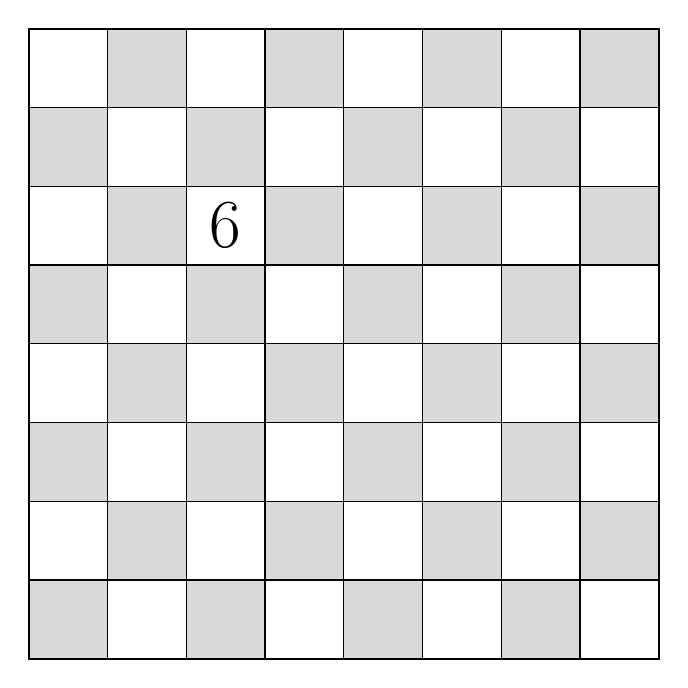
\begin{tikzpicture}[scale=1]
\foreach \row in {0, 2, 4,6}{
  \foreach \col in {0,2,4,6}{
  \draw[fill=gray!30] (\row,\col) rectangle (\row+1, \col+1) rectangle (\row+2, \col+2);
  }
}
\draw[thick] (0,0) rectangle (8,8);
\node at (0.5,7.5) {\Huge \symrook};
\node at (2.5,5.5) {\Huge $6$};
\end{tikzpicture}
\end{center}

\vfill
 \centerline{Math 228 \hfill \textbf{Counting Rook Paths} \hfill Monday, Oct 1}
\vskip 1em
In chess, a rook can move only in straight lines (not diagonally). Fill in each square of the chess board below with the number of different shortest paths the rook, in the upper left corner, can take to get to that square. For example, one square is already filled in. There are six different paths from the rook to the square: DDRR (down down right right), DRDR, DRRD, RDDR, RDRD and RRDD.

\begin{center}
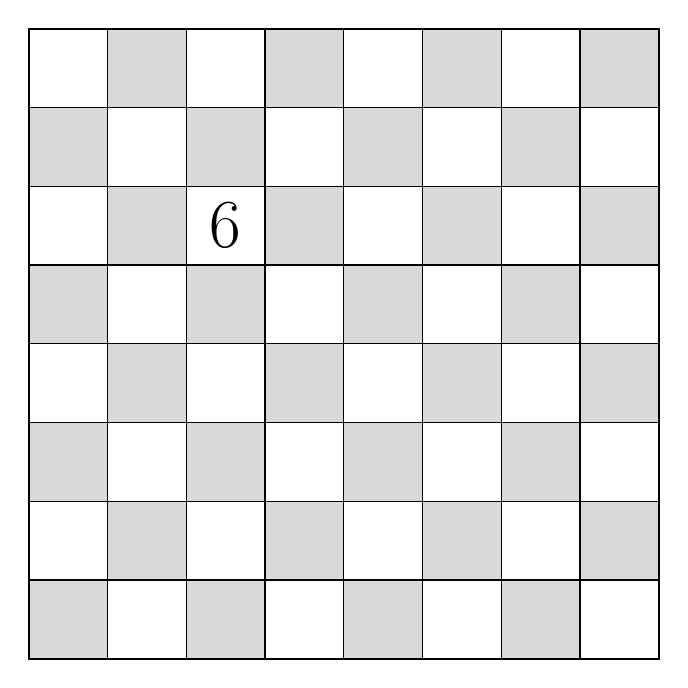
\begin{tikzpicture}[scale=1]
\foreach \row in {0, 2, 4,6}{
  \foreach \col in {0,2,4,6}{
  \draw[fill=gray!30] (\row,\col) rectangle (\row+1, \col+1) rectangle (\row+2, \col+2);
  }
}
\draw[thick] (0,0) rectangle (8,8);
\node at (0.5,7.5) {\Huge \symrook};
\node at (2.5,5.5) {\Huge $6$};
\end{tikzpicture}
\end{center}
\vskip .25in

\clearpage
~
\vskip 1in

\begin{center}
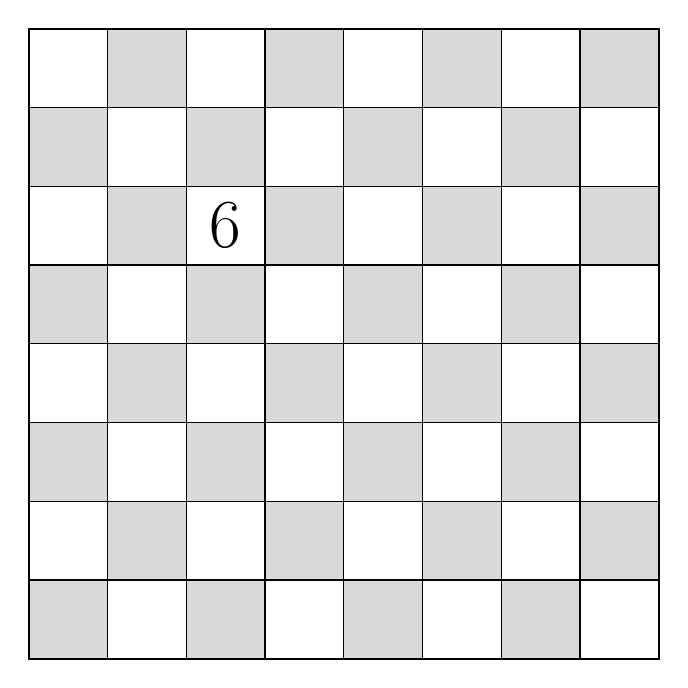
\begin{tikzpicture}[scale=1]
\foreach \row in {0, 2, 4,6}{
  \foreach \col in {0,2,4,6}{
  \draw[fill=gray!30] (\row,\col) rectangle (\row+1, \col+1) rectangle (\row+2, \col+2);
  }
}
\draw[thick] (0,0) rectangle (8,8);
\node at (0.5,7.5) {\Huge \symrook};
\node at (2.5,5.5) {\Huge $6$};
\end{tikzpicture}
\vfill

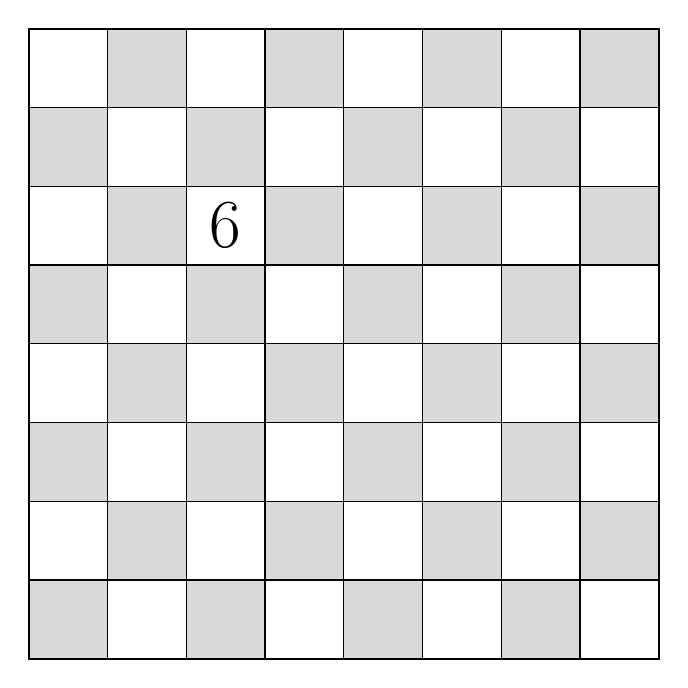
\begin{tikzpicture}[scale=1]
\foreach \row in {0, 2, 4,6}{
  \foreach \col in {0,2,4,6}{
  \draw[fill=gray!30] (\row,\col) rectangle (\row+1, \col+1) rectangle (\row+2, \col+2);
  }
}
\draw[thick] (0,0) rectangle (8,8);
\node at (0.5,7.5) {\Huge \symrook};
\node at (2.5,5.5) {\Huge $6$};
\end{tikzpicture}
\end{center}
\vskip .25in

\end{document}
